\chapter{Proposed solution to problem}\label{ch:proposed-solution-to-problem}
In chapter~\ref{ch:project-problem}, the problem that this project address was outlined along with the reasoning for the
project. This chapter builds upon that giving a format mathematical model of the problem
(section~\ref{sec:optimisation-problem}). While the overall problem is about resource allocation, we believe that cloud
provider would wish to be paid for the use of their services so this additional problem is addressed in
section~\ref{sec:auctioning-of-tasks}. Using these two problems from the previous two sections,
section~\ref{sec:proposed-agents} proposed agents who can learn how to maximise their profit over time.

\section{Resource Allocation Optimisation problem}\label{sec:optimisation-problem}
Using the flexible resource allocation principle presented in~\cite{FlexibleResourceAllocation}, a format mathematical
description of the model can developed. The principle is that for certain resources, the time taken for a operation to occur,
e.g.\ loading of a program, computing the program and sending of results, etc, is proportional to the amount of
resources allocated to completed the operation. \footnote{This principle is not always true, for example, video
decompression is a generally a single thread operation and cannot be effectively multi-threaded. However for this
project we only consider tasks that can be parallelised effectively.}
Therefore instead of allowing the user to requesting a fixed amount of resources for loading, computing and sending back
the results of a program, the user would instead inform the server the total amount of bandwidth required,
computational power, etc for the task to be completed. Then the server can dynamically allocate its available resources
to all of its allocated tasks. This is believed to be effective compared to standard resource allocation mechanism as
bottleneck can occur on certain resource preventing additional tasks from being allocated due servers not
having the requested resources available for the task. Therefore using this principle, a modified version of a standard
resource allocation formulation can be described to maximise social welfare.

A sketch of the system is shown in Fig.~\ref{fig:system_model}.
We assume that in the system there is a set of $I = \{1,2,\ldots,\left|I\right|\}$ servers are heterogeneous in all
characters. Each server has a fixed availability of resources: storage for the code/data needed to run a task
(e.g., measured in GB), computation capacity in terms of CPU cycles per time interval (e.g., measured in FLOP/s),
and communication bandwidth to receive the data and to send back the results of the task after execution
(e.g., measured in Mbit/s). We denote these resources for server $i$: the storage capacity as $S_i$, computation
capacity as $W_i$, and the communication capacity as $R_i$.

\begin{figure}
    \centering
    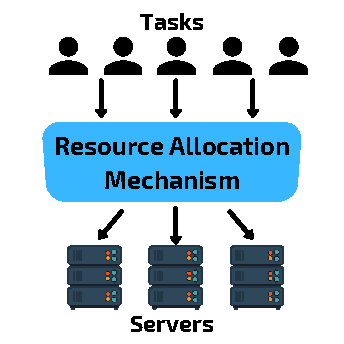
\includegraphics[width=8cm]{figures/system_model.pdf}
    \caption{System model}
    \label{fig:system_model}
\end{figure}

There is a set $J = \{1,2,\ldots,\left| J \right|\}$ of  different tasks that require service from one of the servers
in set $I = \{1,2,\ldots, \left| I \right|\}$. To run any of these tasks on a server requires storing the appropriate
code/data on the same server. These could be, for example, a set of images, videos or CNN layers in identification
tasks. The storage size of task $j$ is denoted as $s_j$ with the rate at which the program is transferred to the server
$i$ at time $t$ being $s^{'}_{i,j,t}$. For a task to be computed successfully, it must fetch and execute instructions
on a CPU. We consider the total number of CPU cycles required for the program to be $w_j$, where the rate at which the
CPU cycles are assigned to the task on server $i$ at time $t$ is $w^{'}_{i,j,t}$. Finally, after the task is run and
the results obtained, the latter need to be sent back to the user. The size of the results for task $j$ is denoted with
$r_j$, and the rate at which they are sent back to the user is $r^{'}_{i,j,t}$ on server $i$ at time $t$. Every task
has a beginning time, denoted by $b_j$ and a deadline, denoted by $d_j$. This is the maximum time for the task to be
completed in order for the user to derive its value. This time includes: the time required to send the data/code to the
server, run it on the server, and get back the results. Therefore for the task to be successfully completed, it must
completed fulfill the constraint in equation~\eqref{eq:deadline}. These operations must occur in order (loading,
computing then sending of results) as a server couldn't compute a task that was not fully loaded on the machine.

\begin{align}
    \frac{s_j}{\sum^{d_j}_{t=b_j} s^{'}_{i,j,t}} + \frac{w_j}{\sum^{d_j}_{t=b_j} w^{'}_{i,j,t}}  +
    \frac{r_j}{\sum^{d_j}_{t=b_j} r^{'}_{i,j,t}} \leq d_j && \forall{j \in J}  \label{eq:deadline}
\end{align}

As server have limited capacity, the total resource usages for all tasks running on a server must be capped.
The storage constraint (equation~\eqref{eq:server_storage_capacity}) is unique as the previous amount
loaded in kept till the end of a program on server. While the computation capacity
(equation~\eqref{eq:server_computation_capacity} is the sum of compute used by all of the tasks on a server $i$ at time $t$ and the
bandwidth capacity (equation~\eqref{eq:server_bandwidth_capacity}) is the sum of loading and sending usages by tasks.
\begin{align}
    \sum_{j \in J} \left(\sum^{d_j}_{t=b_j} s^{'}_{i,j,t} \right) \leq S_i, && \forall{i \in I} \label{eq:server_storage_capacity} \\
    \sum_{j \in J} w^{'}_{i,j,t} \leq W_i, && \forall{i \in I, t \in T} \label{eq:server_computation_capacity} \\
    \sum_{j \in J} s^{'}_{i,j,t} + r^{'}_{i,j,t} \leq R_i, && \forall{i \in I, t \in T} \label{eq:server_bandwidth_capacity} \\
\end{align}

% Todo add complete mathematical description of the problem

\section{Auctioning of Tasks}\label{sec:auctioning-of-tasks}
While the mathematically description of the problem presented above doesn't contain any auctioning properties, in real
life cloud providers normally wish to be paid to the use of their services. However due to the modifications that
this project has to make to the optimisation problems compared to a traditional cloud computing optimisation problem.
All traditional auction mechanisms that have been discussed in section~\ref{sec:related-work-in-cloud-computing} cannot
be used as the user is not requesting a fixed amount of resources nor can the available resources be easily computed
as this is dynamic depending on the currently allocated tasks to a server. This means that a novel or modified auction
mechanism must be used to deal with these changes. Due to the complexities of devising new auction mechanism and the
large corpus of research on auctions already, this project has chosen to use the Vickrey auction~\citep{vickrey}.
This decision is justified in section~\ref{sec:justification-of-vickrey-auction-mechanisms} on why auction over other
alternatives was chosen.

The modification that is made to the Vickrey auction is to reverse the auction as server are bidding on tasks instead of
a task paying servers. Because of this, the auction is referenced to as the reverse Vickrey auction. The auction works
by allowing servers all submit their bid for the task with the winner being the server with the lowest
price but actually only gains second lowest price. The advantage of using the Vickrey auction is that it is  incentive
compatible meaning that the dominant strategy for bidding on a task is to bid your truthful value. This should help
server as they dont need to learn how to outbid another agent as it only needs to consider its own evaluation.
This also allows agents to learn through self-play effectively. The auction also has only a single round of bidding
compared to alternative auctions like English or Dutch auctions. This makes auctioning fast no matter the number of
servers and it also allows for tasks to set a reserve price.

\section{Proposed Agents}\label{sec:proposed-agents}
Using the optimisation formulation and auction problem from the previous two sections, the problem can explained
using the markov decision process format in figure~\ref{fig:mdp_system_model}. The format separates out the auction
parts of the problem and the resource allocation part of the problem with separate agents to act during these
parts of the problem. While the state and action spaces of the agents can be the same, the policies that the agents
will be following are completely different therefore making it impossible to merge the two agents into one.
In subsection~\ref{subsec:proposed-auction-agents} and~\ref{subsec:proposed-resource-allocation-agents} agents are
proposed for the auction environment and resource allocation environment respectively.

\begin{figure}
    \centering
    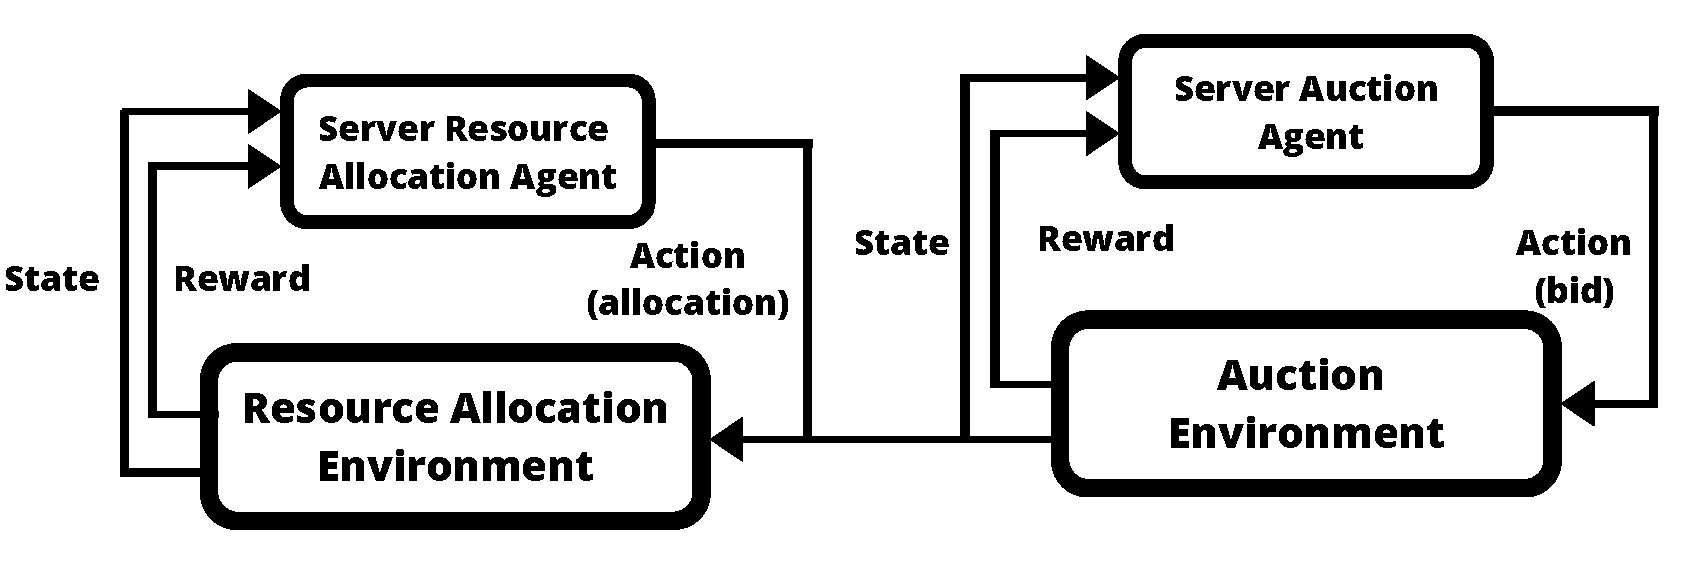
\includegraphics[width=14cm]{figures/flexible_resource_allocation_env.pdf}
    \caption{Markov Decision process system model}
    \label{fig:mdp_system_model}
\end{figure}

The overall problem is of particularly interesting for multi-agent reinforcement learning environment as aim of the
environment is cooperative (to maximise the social welfare) but the servers in competition during the auctions
in order to maximise their profit. But then the server must be cooperative in allocating of resources to each task
as the server wish to complete as many tasks as they can.

\subsection{Proposed auction agents}\label{subsec:proposed-auction-agents}
Traditionally pricing mechanisms~\citep{al2013cloud} rely on mixture of metrics; resource availability, resource demand,
quality of service, task resource requirements, task resource allocation quantity, etc. However these values are
difficult to approximate at the point of server bidding. Due to the complexity of a function to this, reinforcement
learning will be used to learn this function in order to maximise the profits of the server. Simple heuristics will
also be implemented in order compare the effectiveness of the reinforcement learning to untrained heuristics.

As the space of prices, the action space of the agent, is continuous value greater than zero. Therefore a
deep deterministic policy gradient~\citep{ddpg} agent that allows for discrete state spaces and continuous action spaces
will be implemented. Also as the action space can be discretized then several deep Q learning agents will be trained
that use different heuristics in order to compare the results.

These agents will use neural networks, as they function as universal function
approximators~\citep{csaji2001approximation}, for the agents to use to learn. Because of this, a long/short term
memory (LSTM) layer will be used as it allows for multiple inputs and provides a single output that will have
several additional layers to allow additional complexity. With the network ending at a single ReLU neuron for DDPG
or multiple linear activation neurons for DQN agents. The justification for this network over other neural network
models is explained in section~\ref{subsec:justification-for-auctioning-networks}

\subsection{Proposed resource allocation agents}\label{subsec:proposed-resource-allocation-agents}
When a new task is allocated to the server or a task completes a stage then the server resource will be redistributed.
As the problem of how to allocation resources isn't as complex as the agent pricing in
section~\ref{subsec:proposed-auction-agents}, both simple heuristics and reinforcement learning agents will be
implemented in order to compare effectiveness.

However a similar problem exists to the proposed auction agents (in subsection~\ref{subsec:proposed-auction-agents}) as
to know how to allocate resources to be single task is be aware of the other tasks that the server currently contains.
Therefore a similar network is proposed to allow for the other tasks to be passed in in order to compare the current
task having resources allocated to and the other tasks also allocated to the server. The only other change is that
the action space doesn't represent the equivalent amount of a certain type of resources but instead the weighting
for that resources. This is as if the network wanted to allocate as many resources as possible while having to keep
the total amount of resource under the total available then this is extremely difficult. Therefore the action space
instead represents the weight of that resource with the equivalent amount of resources can then be determined by the
server. This aims to reduce the needed complexity of the resource allocation function and speed up the learning time
of the agent.